\documentclass{article}

% packages
\usepackage[margin=.5in]{geometry}
\usepackage{amsmath,amssymb}
\usepackage[none]{hyphenat}
\usepackage{calc}
\usepackage{enumitem}
\usepackage{float}
\usepackage{pgffor}
\usepackage{multirow}
\usepackage[dvipsnames]{xcolor}
\usepackage{hyperref}
\usepackage{tikz}

% details
\author{koku17}
\title{Theory of Computation}

% presets
\hypersetup{
    hidelinks
}
\pagecolor{black}
\color{white}
\usetikzlibrary{
	automata,
	positioning,
	arrows.meta
}

% macros
\definecolor{BrightGreen}{rgb}{.4, 1, 0}
\def\hltt{\color{BrightGreen}}
\newcommand{\module}[1]{
	\phantomsection
	\begin{center}
		\textbf{{\LARGE#1}}
	\end{center}
	\stepcounter{section}
	\addcontentsline{toc}{section}{#1}
}
\newcommand{\que}[2]{
	\item \phantomsection #1
	\addcontentsline{toc}{subsubsection}{#2}
}
\newcommand{\ans}{
	\item [$\longrightarrow$]
}
\newcommand{\indentpar}[2]{
	\begin{itemize}[leftmargin=#1,label=]
		\item #2
	\end{itemize}
}
\newlength{\ansindent}
\setlength{\ansindent}{\widthof{\phantom{$\longrightarrow$}}}

\begin{document}
    \pagenumbering{gobble} \maketitle \newpage
    \pagenumbering{roman} \pdfbookmark[1]{Contents}{} \tableofcontents \newpage
    \pagenumbering{arabic}

	\tikzset{
		node distance=5em,
		every loop/.append style={
			-Straight Barb
		},
		every initial by arrow/.style={
			-Straight Barb
		},
		every edge/.append style={
			-Straight Barb
		},
		initial text=,
		double=black
	}

	\module{Module 1}
	\subsection{Definite Finite State Machines}
	\begin{enumerate}[label=\arabic*)]
		\que{Draw a DFA to accept string of $a$'s having at least one $a$}{~Accept one or more $a$'s}
		\ans
			\begin{enumerate}[label=Step \arabic* :,itemindent=\ansindent]
				\item Minimum String is `$a$'
				\item Alphabets $$\sum=\{a\}$$
				\item Skeleton DFA
					\begin{figure}[H]
	\centering
	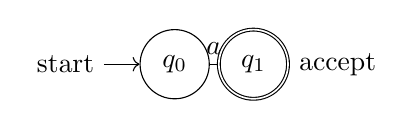
\begin{tikzpicture}
		\draw
			node[state,initial]                                  (q0) {$q_0$}
			node[state,accepting,right of=q0,label=right:accept] (q1) {$q_1$}

			(q0) edge[above] node{$a$} (q1)
		;
	\end{tikzpicture}
\end{figure}

				\item Possible Transitions
					\begin{figure}[H]
	\centering
	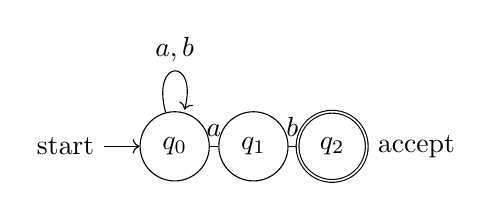
\begin{tikzpicture}
		\draw
			node[state,initial]                                  (q0) {$q_0$}
			node[state,right of=q0]                              (q1) {$q_1$}
			node[state,accepting,right of=q1,label=right:accept] (q2) {$q_2$}

			(q0) edge[above]      node{$a$}   (q1)
			(q0) edge[loop above] node{$a,b$} (q1)
			(q1) edge[above]      node{$b$}   (q2)
		;
	\end{tikzpicture}
\end{figure}

					\begin{table}[H]
						\centering
						\begin{tabular}{l|l}
							$\delta$ & $a$ \\ \hline
							$q_0$ & $q_1$  \\
							$q_1$ & $q_1$
						\end{tabular}
					\end{table}
				\item Final DFA \begin{figure}[H]
	\centering
	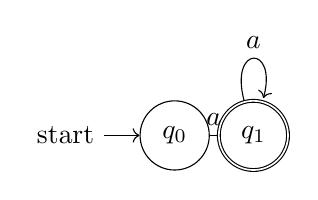
\begin{tikzpicture}
	\draw
		node [state,initial]               (q0) {$q_0$}
		node [state,accepting,right of=q0] (q1) {$q_1$}
		(q0) edge[above] node{$a$}         (q1)
		(q1) edge[loop above] node{$a$}    (q1)
	;
	\end{tikzpicture}
\end{figure}

				\item Language $$\text{L}=\{a^n~|~n\ge1\}$$
			\end{enumerate} \newpage

		\que{Draw a DFA to accept strings of $a$'s and $b$'s having at least one `$a$'}{
			Accept $a$'s and $b$'s with at least one $a$
		}
		\ans
			\begin{enumerate}[label=Step \arabic* :,itemindent=\ansindent]
				\item Minimum String is `$a$'
				\item Alphabets $$\sum=\{a,b\}$$
				\item Skeleton DFA
					\begin{figure}[H]
	\centering
	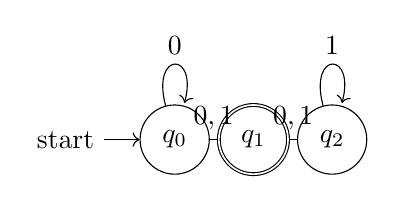
\begin{tikzpicture}
		\draw
			node[state,initial]               (q0) {$q_0$}
			node[state,accepting,right of=q0] (q1) {$q_1$}
			node[state,right of=q1]           (q2) {$q_2$}

			(q0) edge[loop above] node{$0$}   (q0)
			(q2) edge[loop above] node{$1$}   (q2)
			(q0) edge[above]      node{$0,1$} (q1)
			(q1) edge[above]      node{$0,1$} (q2)
		;
	\end{tikzpicture}
\end{figure}

				\item Possible Transitions
					\begin{figure}[H]
	\centering
	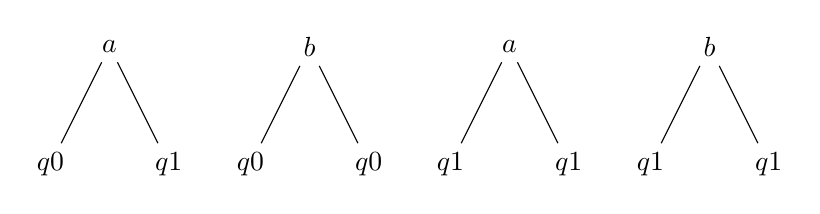
\begin{tikzpicture}[node distance=1in]
		\draw
			node (0) {$a$}
				child {node {$q0$}}
				child {node {$q1$}}

			node[right of=0] (0) {$b$}
				child {node {$q0$}}
				child {node {$q0$}}

			node[right of=0] (0) {$a$}
				child {node {$q1$}}
				child {node {$q1$}}

			node[right of=0] (0) {$b$}
				child {node {$q1$}}
				child {node {$q1$}}
		;
	\end{tikzpicture}
\end{figure}

					\begin{table}[H]
						\centering
						\begin{tabular}{l|l|l}
							$\delta$ & $a$ & $b$  \\ \hline
							$q_0$ & $q_1$ & $q_0$ \\
							$q_1$ & $q_1$ & $q_1$
						\end{tabular}
					\end{table}
				\item Final DFA \begin{figure}[H]
	\centering
	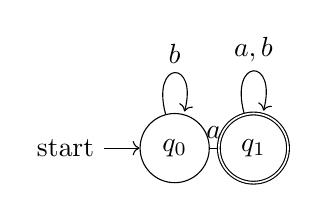
\begin{tikzpicture}
	\draw
		node [state,initial]               (q0) {$q_0$}
		node [state,accepting,right of=q0] (q1) {$q_1$}
		(q0) edge[loop above] node{$b$}    (q0)
		(q0) edge[above] node{$a$}         (q1)
		(q1) edge[loop above] node{$a,b$}  (q1)
	;
	\end{tikzpicture}
\end{figure}

				\item Language $$\text{L}=\{a^n~|~n\ge1\}$$
			\end{enumerate} \newpage

		\que{Draw a DFA to accept strings of $a$'s and  $b$'s having exactly one $a$}{
			Accept an $a$ and $b$'s with exactly one $a$
		}
		\ans
			\begin{enumerate}[label=Step \arabic* :,itemindent=\ansindent]
				\item Minimum String is `$a$'
				\item Alphabets $$\sum=\{a,b\}$$
				\item Skeleton DFA
					\begin{figure}[H]
	\centering
	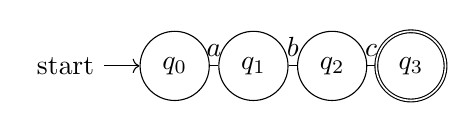
\begin{tikzpicture}
		\draw
			node[state,initial]               (q0) {$q_0$}
			node[state,right of=q0]           (q1) {$q_1$}
			node[state,right of=q1]           (q2) {$q_2$}
			node[state,accepting,right of=q2] (q3) {$q_3$}

			(q0) edge[above] node{$a$} (q1)
			(q1) edge[above] node{$b$} (q2)
			(q2) edge[above] node{$c$} (q3)
		;
	\end{tikzpicture} \\
	$abc$
\end{figure}

\begin{figure}[H]
	\centering
	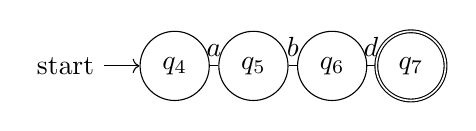
\begin{tikzpicture}
		\draw
			node[state,initial]               (q4) {$q_4$}
			node[state,right of=q4]           (q5) {$q_5$}
			node[state,right of=q5]           (q6) {$q_6$}
			node[state,accepting,right of=q6] (q7) {$q_7$}

			(q4) edge[above] node{$a$} (q5)
			(q5) edge[above] node{$b$} (q6)
			(q6) edge[above] node{$d$} (q7)
		;
	\end{tikzpicture} \\
	$abd$
\end{figure}

\begin{figure}[H]
	\centering
	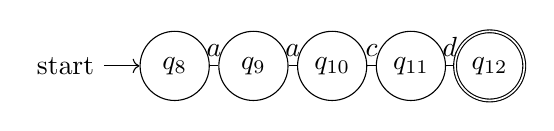
\begin{tikzpicture}
		\draw
			node[state,initial]                (q8)  {$q_8$}
			node[state,right of=q8]            (q9)  {$q_9$}
			node[state,right of=q9]            (q10) {$q_{10}$}
			node[state,right of=q10]           (q11) {$q_{11}$}
			node[state,accepting,right of=q11] (q12) {$q_{12}$}

			(q8)  edge[above] node{$a$} (q9)
			(q9)  edge[above] node{$a$} (q10)
			(q10) edge[above] node{$c$} (q11)
			(q11) edge[above] node{$d$} (q12)
		;
	\end{tikzpicture} \\
	$aacd$
\end{figure}

				\item Possible Transitions
					\begin{figure}[H]
	\centering
	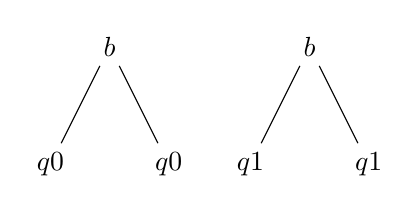
\begin{tikzpicture}[node distance=1in]
		\draw
			node (0) {$b$}
				child {node {$q0$}}
				child {node {$q0$}}

			node[right of=0] (0) {$b$}
				child {node {$q1$}}
				child {node {$q1$}}
		;
	\end{tikzpicture}
\end{figure}

					\begin{table}[H]
						\centering
						\begin{tabular}{l|l|l}
							$\delta$ & $a$ & $b$  \\ \hline
							$q_0$ & $q_1$ & $q_0$ \\
							$q_1$ & $\varnothing$ & $q_1$
						\end{tabular}
					\end{table}
				\item Final DFA
					\begin{figure}[H]
						\centering
							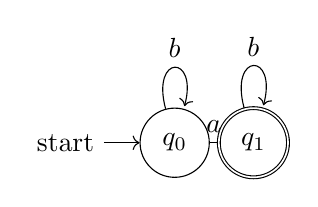
\begin{tikzpicture}
	\draw
		node [state,initial]               (q0) {$q_0$}
		node [state,accepting,right of=q0] (q1) {$q_1$}
		(q0) edge[loop above] node{$b$}    (q0)
		(q0) edge[above] node{$a$}         (q1)
		(q1) edge[loop above] node{$b$}    (q1)
	;
\end{tikzpicture}

							$$\text{OR}$$
							\begin{figure}[H]
	\centering
	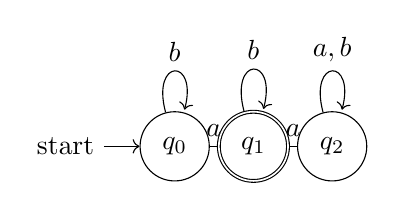
\begin{tikzpicture}
	\draw
		node [state,initial]               (q0) {$q_0$}
		node [state,accepting,right of=q0] (q1) {$q_1$}
		node [state,right of=q1]           (q2) {$q_2$}
		(q0) edge[loop above] node{$b$}    (q0)
		(q0) edge[above] node{$a$}         (q1)
		(q1) edge[loop above] node{$b$}    (q1)
		(q1) edge[above] node{$a$}         (q2)
		(q2) edge[loop above] node{$a,b$}  (q2)
	;
	\end{tikzpicture}
\end{figure}

					\end{figure}
				\item Language $$\text{L}=\{ab^n~|~n\ge0\}$$
			\end{enumerate} \newpage

		\que{Obtain a DFA to accept strings of $a$'s and $b$'s starting with the string $ab$}{
			Accept $a$'s and $b$'s starting with $ab$
		}
		\ans
			\begin{enumerate}[label=Step \arabic* :,itemindent=\ansindent]
				\item Minimum String is `$ab$'
				\item Alphabets $$\sum=\{a,b\}$$
				\item Skeleton DFA
					\begin{figure}[H]
	\centering
	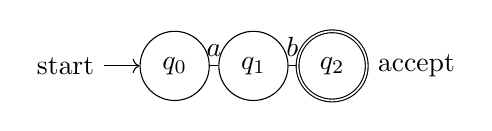
\begin{tikzpicture}
	\draw
		node [state,initial]                                  (q0) {$q_0$}
		node [state,right of=q0]                              (q1) {$q_1$}
		node [state,accepting,right of=q1,label=right:accept] (q2) {$q_2$}
		(q0) edge[above] node{$a$}                            (q1)
		(q1) edge[above] node{$b$}                            (q2)
	;
	\end{tikzpicture}
\end{figure}

				\item Possible Transitions
					\begin{figure}[H]
	\centering
	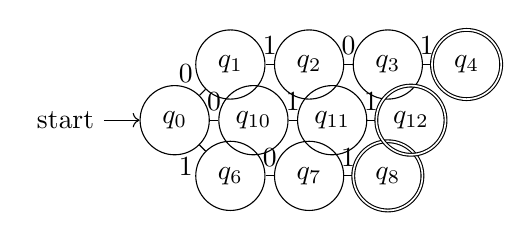
\begin{tikzpicture}
		\draw
			node[state,initial]                (q0) {$q_0$}
			node[state,above right of=q0]      (q1) {$q_1$}
			node[state,right of=q1]            (q2) {$q_2$}
			node[state,right of=q2]            (q3) {$q_3$}
			node[state,accepting,right of=q3]  (q4) {$q_4$}

			node[state,below right of=q0]      (q6) {$q_6$}
			node[state,right of=q6]            (q7) {$q_7$}
			node[state,accepting,right of=q7]  (q8) {$q_8$}

			node[state,right of=q0]            (q10) {$q_{10}$}
			node[state,right of=q10]           (q11) {$q_{11}$}
			node[state,accepting,right of=q11] (q12) {$q_{12}$}

			(q0)  edge[above left] node{$0$} (q1)
			(q1)  edge[above]      node{$1$} (q2)
			(q2)  edge[above]      node{$0$} (q3)
			(q3)  edge[above]      node{$1$} (q4)

			(q0)  edge[above]      node{$0$} (q10)
			(q6)  edge[above]      node{$0$} (q7)
			(q7)  edge[above]      node{$1$} (q8)

			(q0)  edge[below left] node{$1$} (q6)
			(q10) edge[above]      node{$1$} (q11)
			(q11) edge[above]      node{$1$} (q12)
		;
	\end{tikzpicture}
\end{figure}


					\begin{table}[H]
						\centering
						\begin{tabular}{l|l|l}
							$\delta$ & $a$ & $b$          \\ \hline
							$q_0$ & $q_1$ & $\varnothing$ \\
							$q_1$ & $\varnothing$ & $q_2$ \\
							$q_2$ & $q_2$ & $q_2$
						\end{tabular}
					\end{table}
				\item Final DFA \begin{figure}[H]
	\centering
	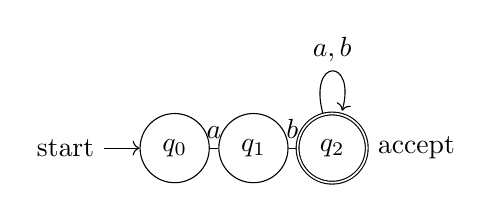
\begin{tikzpicture}
	\draw
		node [state,initial]                                  (q0) {$q_0$}
		node [state,right of=q0]                              (q1) {$q_1$}
		node [state,accepting,right of=q1,label=right:accept] (q2) {$q_2$}
		(q0) edge[above] node{$a$}                            (q1)
		(q1) edge[above] node{$b$}                            (q2)
		(q2) edge[loop above] node{$a,b$}                     (q2)
	;
	\end{tikzpicture}
\end{figure}

				\item Language $$\text{L}=\{ab\text{W}^n~|~\text{W}\in\{a,b\},n\ge0~\}$$
			\end{enumerate} \newpage

		\que{Draw DFA to accept strings of $a$'s and $b$'s ending with the string $abb$}{
			Accept strings of $a$'s and $b$'s ending with $abb$
		}
		\ans
			\begin{enumerate}[label=Step \arabic* :,itemindent=\ansindent]
				\item Minimum String is `$abb$'
				\item Alphabets $$\sum=\{a,b\}$$
				\item Skeleton DFA
					\begin{figure}[H]
    \centering
    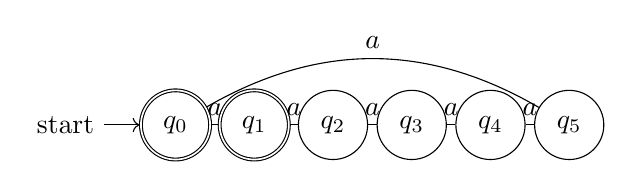
\begin{tikzpicture}
		\draw
			node [state,accepting,initial]     (q0) {$q_0$}
			node [state,accepting,right of=q0] (q1) {$q_1$}
			node [state,right of=q1]           (q2) {$q_2$}
			node [state,right of=q2]           (q3) {$q_3$}
			node [state,right of=q3]           (q4) {$q_4$}
			node [state,right of=q4]           (q5) {$q_5$}

			(q0) edge [above]            node{$a$} (q1)
			(q1) edge [above]            node{$a$} (q2)
			(q2) edge [above]            node{$a$} (q3)
			(q3) edge [above]            node{$a$} (q4)
			(q4) edge [above]            node{$a$} (q5)
			(q5) edge [above,bend right] node{$a$} (q0)
		;
    \end{tikzpicture}
\end{figure}

				\item Possible Transitions
					\begin{figure}[H]
    \centering
    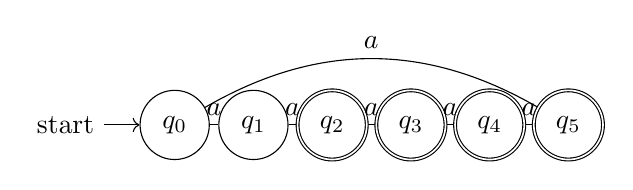
\begin{tikzpicture}
		\draw
			node[state,initial]               (q0) {$q_0$}
			node[state,right of=q0]           (q1) {$q_1$}
			node[state,accepting,right of=q1] (q2) {$q_2$}
			node[state,accepting,right of=q2] (q3) {$q_3$}
			node[state,accepting,right of=q3] (q4) {$q_4$}
			node[state,accepting,right of=q4] (q5) {$q_5$}

			(q0) edge[above]            node{$a$} (q1)
			(q1) edge[above]            node{$a$} (q2)
			(q2) edge[above]            node{$a$} (q3)
			(q3) edge[above]            node{$a$} (q4)
			(q4) edge[above]            node{$a$} (q5)
			(q5) edge[above,bend right] node{$a$} (q0)
		;
    \end{tikzpicture}
\end{figure}

					\begin{table}[H]
						\centering
						\begin{tabular}{l|l|l}
							$\delta$ & $a$ & $b$  \\ \hline
							$q_0$ & $q_1$ & $q_0$ \\
							$q_1$ & $q_1$ & $q_2$ \\
							$q_2$ & $q_2$ & $q_3$ \\
							$q_3$ & $q_1$ & $q_0$
						\end{tabular}
					\end{table}
				\item Final DFA \begin{figure}[H]
	\centering
	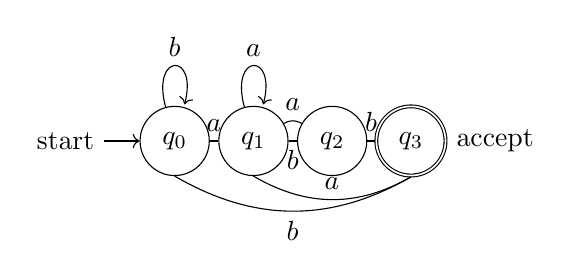
\begin{tikzpicture}
	\draw
		node [state,initial]                                  (q0) {$q_0$}
		node [state,right of=q0]                              (q1) {$q_1$}
		node [state,right of=q1]                              (q2) {$q_2$}
		node [state,accepting,right of=q2,label=right:accept] (q3) {$q_3$}
		(q0) edge[above] node{$a$} (q1)
		(q1) edge[below] node{$b$} (q2)
		(q2) edge[above] node{$b$} (q3)

		(q0) edge[loop above] node{$b$}            (q0)
		(q1) edge[loop above] node{$a$}            (q1)
		(q2) edge[bend right,above] node{$a$}      (q1)
		(q3.south) edge[bend left,above] node{$a$} (q1.south)
		(q3.south) edge[bend left,below] node{$b$} (q0.south)
	;
	\end{tikzpicture}
\end{figure}

				\item Language $$\text{L}=\{\text{W}^nabb~|~\text{W}\in\{a,b\},n\ge0~\}$$
			\end{enumerate} \newpage

		\que{Draw DFA to accept strings of $a$'s and $b$'s not ending with the string $abb$}{
			Accept strings of $a$'s and $b$'s not ending with $abb$
		}
		\ans
			\begin{enumerate}[label=Step \arabic* :,itemindent=\ansindent]
				\item Minimum String is `$abb$'
				\item Alphabets $$\sum=\{a,b\}$$
				\item Skeleton DFA
					\begin{figure}[H]
	\centering
	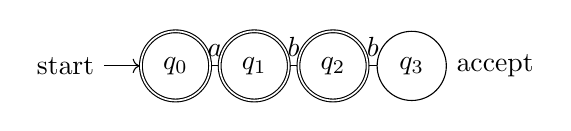
\begin{tikzpicture}
		\draw
			node[state,initial,accepting]              (q0) {$q_0$}
			node[state,accepting,right of=q0]          (q1) {$q_1$}
			node[state,accepting,right of=q1]          (q2) {$q_2$}
			node[state,right of=q2,label=right:accept] (q3) {$q_3$}

			(q0) edge[above] node{$a$} (q1)
			(q1) edge[above] node{$b$} (q2)
			(q2) edge[above] node{$b$} (q3)
		;
	\end{tikzpicture}
\end{figure}

				\item Possible Transitions
					\begin{figure}[H]
	\centering
	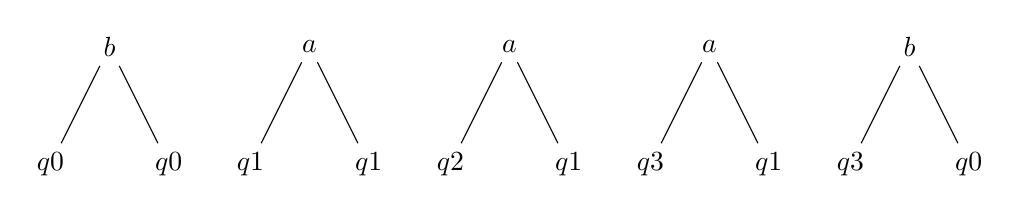
\begin{tikzpicture}[node distance=1in]
		\draw
			node (0) {$b$}
				child {node {$q0$}}
				child {node {$q0$}}

			node[right of=0] (0) {$a$}
				child {node {$q1$}}
				child {node {$q1$}}

			node[right of=0] (0) {$a$}
				child {node {$q2$}}
				child {node {$q1$}}

			node[right of=0] (0) {$a$}
				child {node {$q3$}}
				child {node {$q1$}}

			node[right of=0] (0) {$b$}
				child {node {$q3$}}
				child {node {$q0$}}
		;
	\end{tikzpicture}
\end{figure}

					\begin{table}[H]
						\centering
						\begin{tabular}{l|l|l}
							$\delta$ & $a$ & $b$  \\ \hline
							$q_0$ & $q_1$ & $q_0$ \\
							$q_1$ & $q_1$ & $q_2$ \\
							$q_2$ & $q_2$ & $q_3$ \\
							$q_3$ & $q_1$ & $q_0$
						\end{tabular}
					\end{table}
				\item Final DFA \begin{figure}[H]
	\centering
	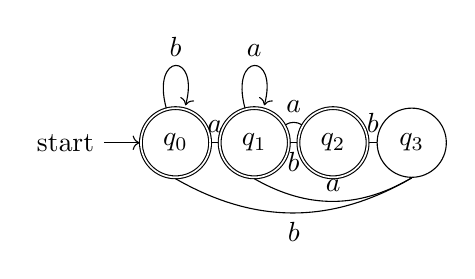
\begin{tikzpicture}
		\draw
			node[state,accepting,initial]     (q0) {$q_0$}
			node[state,accepting,right of=q0] (q1) {$q_1$}
			node[state,accepting,right of=q1] (q2) {$q_2$}
			node[state,right of=q2]           (q3) {$q_3$}

			(q0) edge[above] node{$a$} (q1)
			(q1) edge[below] node{$b$} (q2)
			(q2) edge[above] node{$b$} (q3)

			(q0)       edge[loop above]       node{$b$} (q0)
			(q1)       edge[loop above]       node{$a$} (q1)
			(q2)       edge[bend right,above] node{$a$} (q1)
			(q3.south) edge[bend left,above]  node{$a$} (q1.south)
			(q3.south) edge[bend left,below]  node{$b$} (q0.south)
		;
	\end{tikzpicture}
\end{figure}

				\item Language $$\text{L}=\{\text{W}^nabb~|~\text{W}\in\{a,b\},n\ge0~\}$$
			\end{enumerate} \newpage

		\que{Draw a DFA to accept string of $a$'s \& $b$'s ending with $ab$ or $ba$}{
			Accept string of $a$'s \& $b$'s ending with $ab$ or $ba$
		}
		\ans
			\begin{enumerate}[label=Step \arabic* :,itemindent=\ansindent]
				\item Minimum string is `$ab$' or `$ba$'
				\item Alphabets $$\sum=\{a,b\}$$
				\item Skeleton DFA 
					\begin{figure}[H]
	\centering
	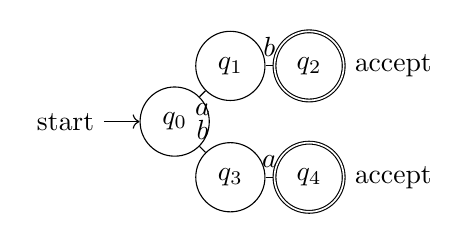
\begin{tikzpicture}
		\draw
			node[state,initial]                                  (q0) {$q_0$}
			node[state,above right of=q0]                        (q1) {$q_1$}
			node[state,below right of=q0]                        (q3) {$q_3$}
			node[state,accepting,right of=q1,label=right:accept] (q2) {$q_2$}
			node[state,accepting,right of=q3,label=right:accept] (q4) {$q_4$}

			(q0) edge[below] node{$a$} (q1)
			(q0) edge[above] node{$b$} (q3)
			(q1) edge[above] node{$b$} (q2)
			(q3) edge[above] node{$a$} (q4)
		;
	\end{tikzpicture}
\end{figure}

				\item Possible Transitions
					\begin{figure}[H]
	\centering
	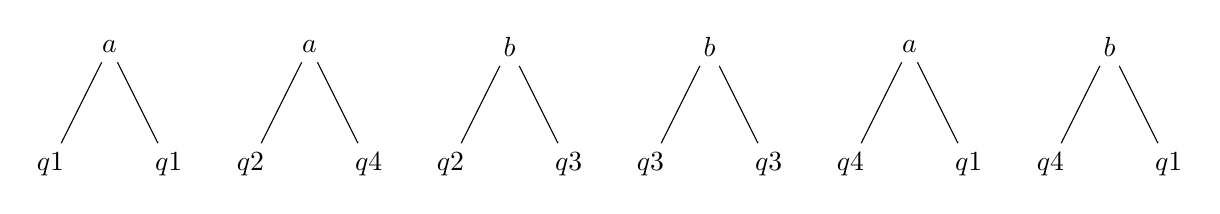
\begin{tikzpicture}[node distance=1in]
		\draw
			node (0) {$a$}
				child {node {$q1$}}
				child {node {$q1$}}

			node[right of=0] (0) {$a$}
				child {node {$q2$}}
				child {node {$q4$}}

			node[right of=0] (0) {$b$}
				child {node {$q2$}}
				child {node {$q3$}}

			node[right of=0] (0) {$b$}
				child {node {$q3$}}
				child {node {$q3$}}

			node[right of=0] (0) {$a$}
				child {node {$q4$}}
				child {node {$q1$}}

			node[right of=0] (0) {$b$}
				child {node {$q4$}}
				child {node {$q1$}}
		;
	\end{tikzpicture}
\end{figure}

					\begin{table}[H]
						\centering
						\begin{tabular}{l|l|l}
							$\delta$ & $a$ & $b$  \\ \hline
							$q_0$ & $q_1$ & $q_3$ \\
							$q_1$ & $q_1$ & $q_2$ \\
							$q_2$ & $q_4$ & $q_3$ \\
							$q_3$ & $q_4$ & $q_3$ \\
							$q_4$ & $q_1$ & $q_2$
						\end{tabular}
					\end{table}
				\item Final DFA \begin{figure}[H]
	\centering
	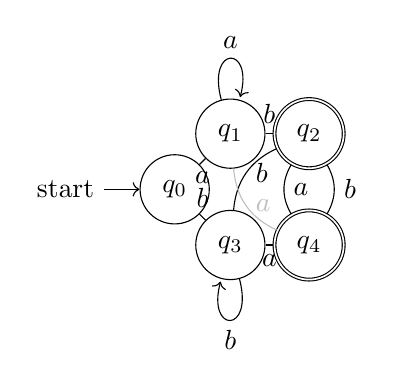
\begin{tikzpicture}
	\draw
		node [state,initial]               (q0) {$q_0$}
		node [state,above right of=q0]     (q1) {$q_1$}
		node [state,below right of=q0]     (q3) {$q_3$}
		node [state,accepting,right of=q1] (q2) {$q_2$}
		node [state,accepting,right of=q3] (q4) {$q_4$}

		(q0) edge[below]                            node{$a$}        (q1)
		(q0) edge[above]                            node{$b$}        (q3)
		(q1) edge[above]                            node{$b$}        (q2)
		(q3) edge[below]                            node{$a$}        (q4)
		(q1) edge[loop above]                       node{$a$}        (q1)
		(q3) edge[loop below]                       node{$b$}        (q3)
		(q2) edge[right,bend right]                 node{$a$}        (q4)
		(q4) edge[right,bend right]                 node{$b$}        (q2)
		(q2) edge[midway,bend right]                node[right]{$b$} (q3)
		(q4) edge[color=lightgray,midway,bend left] node[right]{$a$} (q1)
	;
	\end{tikzpicture}
\end{figure}

				\item Language $$\text{L}=\{\text{W}^n(ab+ba)~|~\text{W}\in\{a,b\},n\ge0~\}$$
			\end{enumerate} \newpage

	\que{
		Draw a DFA to accept set of all strings on the alphabet $\displaystyle \sum=\{0,1\}$ that either
		beings or ends or both with substring 01
	}{
		Accept string starting or ending with $01$
	}
	\ans
		\begin{enumerate}[label=Step \arabic* :,itemindent=\ansindent]
			\item Minimum string is `01'
			\item Alphabets $$\sum=\{0,1\}$$
			\item Skeleton DFA's 
				\begin{figure}[H]
	\centering
	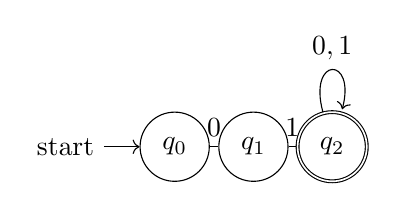
\begin{tikzpicture}
	\draw
		node [state,initial]               (q0) {$q_0$}
		node [state,right of=q0]           (q1) {$q_1$}
		node [state,accepting,right of=q1] (q2) {$q_2$}

		(q0) edge[above] node{$0$}        (q1)
		(q1) edge[above] node{$1$}        (q2)
		(q2) edge[loop above] node{$0,1$} (q2)
	;
	\end{tikzpicture} \\
	Strings starting with $01$
\end{figure}

\begin{figure}[H]
	\centering
	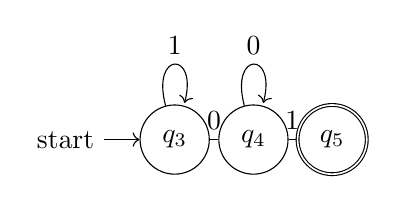
\begin{tikzpicture}
	\draw
		node [state,initial]               (q3) {$q_3$}
		node [state,right of=q3]           (q4) {$q_4$}
		node [state,accepting,right of=q4] (q5) {$q_5$}

		(q3) edge[above] node{$0$}      (q4)
		(q3) edge[loop above] node{$1$} (q4)
		(q4) edge[above] node{$1$}      (q5)
		(q4) edge[loop above] node{$0$} (q5)
	;
	\end{tikzpicture} \\
	Strings ending with $01$
\end{figure}

			\item Combining Transitions
				\begin{figure}[H]
	\centering
	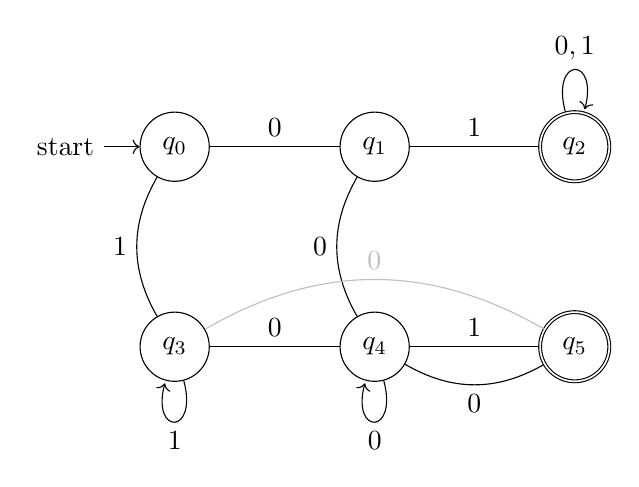
\begin{tikzpicture}[node distance=1in]
		\draw
			node[state,initial]               (q0) {$q_0$}
			node[state,right of=q0]           (q1) {$q_1$}
			node[state,accepting,right of=q1] (q2) {$q_2$}

			node[state,below of=q0]           (q3) {$q_3$}
			node[state,right of=q3]           (q4) {$q_4$}
			node[state,accepting,right of=q4] (q5) {$q_5$}

			(q0) edge[above]      node{$0$}   (q1)
			(q1) edge[above]      node{$1$}   (q2)
			(q2) edge[loop above] node{$0,1$} (q2)

			(q3) edge[above]      node{$0$} (q4)
			(q3) edge[loop below] node{$1$} (q4)
			(q4) edge[above]      node{$1$} (q5)
			(q4) edge[loop below] node{$0$} (q5)

			(q0) edge[left,bend right]                  node{$1$} (q3)
			(q1) edge[left,bend right]                  node{$0$} (q4)
			(q5) edge[below,bend left]                  node{$0$} (q4)
			(q5) edge[color=lightgray,above,bend right] node{$0$} (q3)
		;
	\end{tikzpicture} \\
	Combination of two states
\end{figure}

				\begin{table}[H]
					\centering
					\begin{tabular}{l|l|l}
						$\delta$ & $a$ & $b$  \\ \hline
						$q_0$ & $q_1$ & $q_3$ \\
						$q_1$ & $q_4$ & $q_2$ \\
						$q_2$ & $q_2$ & $q_2$ \\
						$q_3$ & $q_4$ & $q_3$ \\
						$q_4$ & $q_4$ & $q_5$ \\
						$q_5$ & $q_4$ & $q_3$
					\end{tabular}
				\end{table}
		\end{enumerate} \newpage

	\que{Draw a DFA to accept the language $\text{L}=\{\text{W}:n_a(\text{W})\ge1,n_b(\text{W})=2\}$}{
		Accept the language $\text{L}=\{\text{W}:n_a(\text{W})\ge1,n_b(\text{W})=2\}$
	}
	\ans String should have exactly two $b$'s and at least one $a$'s
		\begin{enumerate}[label=Step \arabic* :,itemindent=\ansindent]
			\item Minimum String is $abb,bab,bba$
			\item Skeleton DFA's 
				\begin{figure}[H]
	\centering
	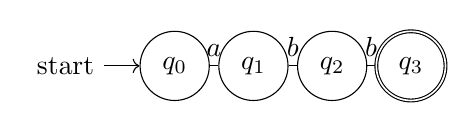
\begin{tikzpicture}
		\draw
			node[state,initial]               (q0) {$q_0$}
			node[state,right of=q0]           (q1) {$q_1$}
			node[state,right of=q1]           (q2) {$q_2$}
			node[state,accepting,right of=q2] (q3) {$q_3$}

			(q0) edge[above] node{$a$}        (q1)
			(q1) edge[above] node{$b$}        (q2)
			(q2) edge[above] node{$b$}        (q3)
		;
	\end{tikzpicture} \\
	Strings starting with $abb$
\end{figure}

\begin{figure}[H]
	\centering
	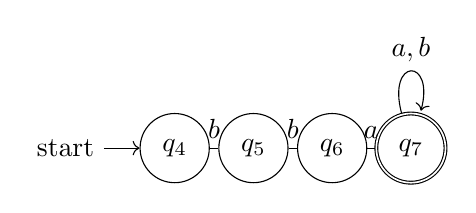
\begin{tikzpicture}
		\draw
			node[state,initial]               (q4) {$q_4$}
			node[state,right of=q4]           (q5) {$q_5$}
			node[state,right of=q5]           (q6) {$q_6$}
			node[state,accepting,right of=q6] (q7) {$q_7$}

			(q4) edge[above]      node{$b$}   (q5)
			(q5) edge[above]      node{$b$}   (q6)
			(q6) edge[above]      node{$a$}   (q7)
			(q7) edge[loop above] node{$a,b$} (q7)
		;
	\end{tikzpicture} \\
	Strings starting with $bba$
\end{figure}

			\item Combining Transitions
				\begin{figure}[H]
	\centering
	\begin{tikzpicture}
		\draw
			node [state,initial]               (q0) {$q_0$}
			node [state,above right of=q0]     (q1) {$q_1$}
			node [state,right of=q1]           (q2) {$q_2$}
			node [state,accepting,right of=q2] (q3) {$q_3$}
			node [state,below right of=q4]     (q4) {$q_4$}
			node [state,right of=q4]           (q5) {$q_5$}
			node [state,right of=q5]           (q6) {$q_6$}

			(q0) edge[below]      node{$a$}   (q1)
			(q1) edge[above]      node{$b$}   (q2)
			(q2) edge[above]      node{$b$}   (q3)

			(q0) edge[above]      node{$b$}   (q4)
			(q4) edge[above]      node{$b$}   (q5)
			(q5) edge[above]      node{$b$}   (q6)

			(q3) edge[loop above] node{$a$}   (q3)
			(q6) edge[loop below] node{$a,b$} (q6)
			(q4) edge[left]       node{$a$}   (q2)
			(q5) edge[left]       node{$a$}   (q3)
			(q3) edge[right]      node{$b$}   (q6)
		;
	\end{tikzpicture} \\
	Combination of two states
\end{figure}

				\begin{table}[H]
					\centering
					\begin{tabular}{l|l|l}
						$\delta$ & $a$ & $b$  \\ \hline
						$q_0$ & $q_1$ & $q_4$ \\
						$q_1$ & $\varnothing$ & $q_2$ \\
						$q_2$ & $\varnothing$ & $q_3$ \\
						$q_3$ & $q_3$ & $q_6$ \\
						$q_4$ & $q_2$ & $q_5$ \\
						$q_5$ & $q_3$ & $q_5$
					\end{tabular}
				\end{table}
		\end{enumerate}
	\end{enumerate} \newpage
	\subsection{Divisible by $k$ problems}
	\begin{enumerate}[label=\arabic*)]
		\que{
			Construct a DFA which accepts string of $0$'s and $1$'s where the value of each string is
			represented as a binary number. Only the strings representing zero modulo 5 should be accepted
		}{~Accept the string starting with $0$'s and $1$'s}
		\ans
		\begin{enumerate}[label=Step \arabic* :,itemindent=\ansindent]
			\item Identify the radix, input alphabets and the divisor
				\begin{align*}
					r&=2 \\
					d&=\{0,1\} \\
					k&=5
				\end{align*}
			\item Compute Possible remainders \\ $i=\{0,1,2,3,4\}$
			\item Compute Transitions
				\begin{table}[H]
					\centering
					\begin{tabular}{|c|c|c|c|} \hline
						$i$ & $d$ & $j$ & $\delta(q_i,d)=q_j$ \\ \hline
						\multirow{2}*{0} & 0 & 0 & $\delta(q_0,0)=q_0$ \\ \cline{2-4}
							& 1 & 1 & $\delta(q_0,1)=q_1$ \\ \hline
						\multirow{2}*{1} & 0 & 2 & $\delta(q_1,0)=q_2$ \\ \cline{2-4}
							& 1 & 3 & $\delta(q_1,1)=q_3$ \\ \hline
						\multirow{2}*{2} & 0 & 4 & $\delta(q_2,0)=q_4$ \\ \cline{2-4}
							& 1 & 0 & $\delta(q_2,1)=q_0$ \\ \hline
						\multirow{2}*{3} & 0 & 1 & $\delta(q_3,0)=q_1$ \\ \cline{2-4}
							& 1 & 2 & $\delta(q_3,1)=q_2$ \\ \hline
						\multirow{2}*{4} & 0 & 3 & $\delta(q_4,0)=q_3$ \\ \cline{2-4}
							& 1 & 4 & $\delta(q_4,1)=q_4$ \\ \hline
					\end{tabular}
				\end{table}
			\item Final DFA
				\begin{figure}[H]
    \centering
    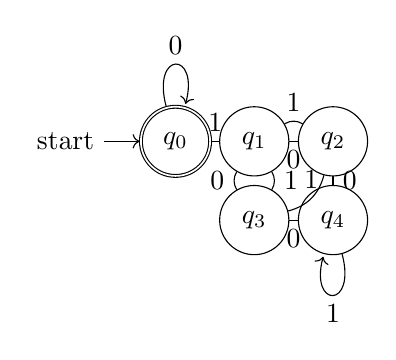
\begin{tikzpicture}
    \draw
        node [state,initial,accepting] (q0) {$q_0$}
        node [state,right of=q0] (q1) {$q_1$}
        node [state,right of=q1] (q2) {$q_2$}
        node [state,below of=q1] (q3) {$q_3$}
        node [state,right of=q3] (q4) {$q_4$}

		(q0) edge[loop above] node{0} (q0)
		(q0) edge[above] node{1} (q1)
		(q1) edge[below] node{0} (q2)
		(q1) edge[right,bend left] node{1} (q3)
		(q2) edge[right] node{0} (q4)
		(q2) edge[above,bend right] node{1} (q1)
		(q3) edge[left,bend left] node{0} (q1)
		(q3) edge[above,bend right] node{1} (q2)
		(q4) edge[below] node{0} (q3)
		(q4) edge[loop below] node{1} (q4)
    ;
    \end{tikzpicture}
\end{figure}

		\end{enumerate} \newpage

		\que{Draw a DFA to accept decimal strings divisible by 3}{
			Accept decimal strings divisible by 3 by method of Counter DFA
		}
		\ans
			\begin{enumerate}[label=Step \arabic* :,itemindent=\ansindent]
				\item Identify the radix, input alphabets and the divisor
					\begin{align*}
						r&=10 \\
						d&=\{0,1,2,3,4,5,6,7,8,9\} \\
						k&=3
					\end{align*}
				\item Compute Possible remainders \\ $i=\{0,1,2\}$
				\item Compute Transitions
					\begin{table}[H]
						\centering
						\begin{tabular}{cc}
							\begin{tabular}{|c|c|c|c|} \hline
								$i$ & $d$ & $j$ & $\delta(q_i,d)=q_j$ \\ \hline
								\multirow{3}*{0} & 0 & 0 & $\delta(q_0,0)=q_0$ \\ \cline{2-4}
									& 1 & 1 & $\delta(q_0,1)=q_1$ \\ \cline{2-4}
									& 2 & 2 & $\delta(q_0,2)=q_2$ \\ \hline 
								\multirow{3}*{1} & 0 & 1 & $\delta(q_1,0)=q_1$ \\ \cline{2-4}
									& 1 & 2 & $\delta(q_1,1)=q_2$ \\ \cline{2-4}
									& 2 & 0 & $\delta(q_1,2)=q_0$ \\ \hline 
								\multirow{3}*{2} & 0 & 2 & $\delta(q_2,0)=q_2$ \\ \cline{2-4}
									& 1 & 0 & $\delta(q_2,1)=q_0$ \\ \cline{2-4}
									& 2 & 1 & $\delta(q_2,2)=q_1$ \\ \hline 
								\multirow{3}*{3} & 0 & 0 & $\delta(q_3,0)=q_0$ \\ \cline{2-4}
									& 1 & 1 & $\delta(q_3,1)=q_1$ \\ \cline{2-4}
									& 2 & 2 & $\delta(q_3,2)=q_2$ \\ \hline
							\end{tabular} &
							\begin{tabular}{lll}
								$\delta(q_0\{0,3,6,9\})$ & $=$ & $q_0$ \\
								$\delta(q_0\{1,4,7\})$   & $=$ & $q_1$ \\
								$\delta(q_0\{2,5,8\})$   & $=$ & $q_2$ \\
								$\delta(q_1\{0,3,6,9\})$ & $=$ & $q_1$ \\
								$\delta(q_1\{1,4,7\})$   & $=$ & $q_2$ \\
								$\delta(q_1\{2,5,8\})$   & $=$ & $q_0$ \\
								$\delta(q_2\{0,3,6,9\})$ & $=$ & $q_2$ \\
								$\delta(q_2\{1,4,7\})$   & $=$ & $q_0$ \\
								$\delta(q_2\{2,5,8\})$   & $=$ & $q_1$
							\end{tabular} \\ ~\vspace{-.5em} \\
							Transitions & Counter DFA
						\end{tabular}
					\end{table}
				\item Final DFA
					\begin{figure}[H]
    \centering
    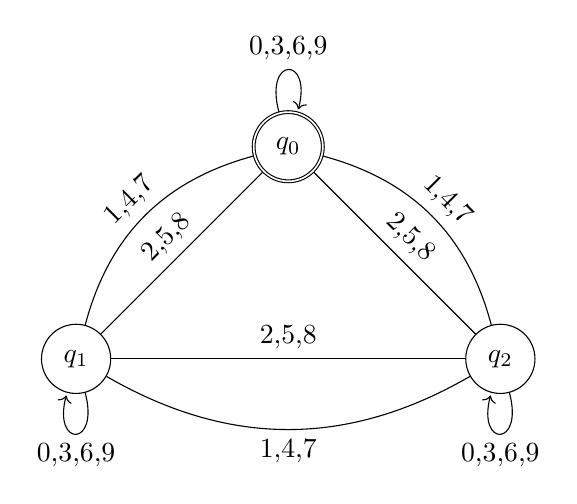
\begin{tikzpicture}[node distance=1.5in]
		\draw
			node[state,accepting]         (q0) {$q_0$}
			node[state,below left of=q0]  (q1) {$q_1$}
			node[state,below right of=q0] (q2) {$q_2$}

			(q0) edge[loop above]       node{0,3,6,9}           (q0)
			(q0) edge[above,bend right] node[rotate=45]{1,4,7}  (q1)
			(q0) edge[above]            node[rotate=-45]{2,5,8} (q2)
			(q1) edge[loop below]       node{0,3,6,9}           (q1)
			(q1) edge[below,bend right] node{1,4,7}             (q2)
			(q1) edge[above]            node[rotate=45]{2,5,8}  (q0)
			(q2) edge[loop below]       node{0,3,6,9}           (q2)
			(q2) edge[above,bend right] node[rotate=-45]{1,4,7} (q0)
			(q2) edge[above]            node{2,5,8}             (q1)
		;
    \end{tikzpicture}
\end{figure}

			\end{enumerate} \newpage

		\que{Obtain DFA to accept strings of even number of $a$'s}{~Accept even number of $a$'s}
		\ans
			\begin{enumerate}[label=Step \arabic* :,itemindent=\ansindent]
				\item Identify the number of states
				\indentpar{1.5em}{Since Even numbers can be 0 and multiple of 2, there would be two states.}
				\item Identify first and final states
					\begin{itemize}[leftmargin=2.5em]
						\item When the number of $a$'s is odd and next $a$ goes to even state
						\item When the number of $a$'s is even and next $a$ goes to odd state 
					\end{itemize}
				\item Compute Transitions
					\begin{table}[H]
						\centering
						\begin{tabular}{cc}
							\begin{tabular}{c|c}
								$\delta$ & $a$ \\ \hline
								E & O \\
								O & E
							\end{tabular} &
							\begin{tabular}{lll}
								$\delta(\text{O},a)$ & $=$ & E \\
								$\delta(\text{E},a)$ & $=$ & O
							\end{tabular}
						\end{tabular}
					\end{table}
				\item Final Design \begin{figure}[H]
    \centering
    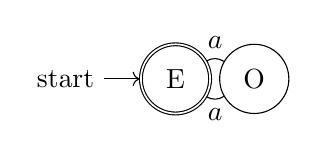
\begin{tikzpicture}
		\draw
			node[state,accepting,initial] (q0) {E}
			node[state,right of=q0]       (q1) {O}

			(q0) edge[above,bend left] node{$a$} (q1)
			(q1) edge[below,bend left] node{$a$} (q0)
		;
    \end{tikzpicture}
\end{figure}

			\end{enumerate}

		\que{
			Obtain a DFA to accept the language $\text{L}=\{\text{W}:|\text{W}|\mod3=0\}$ where
			$\displaystyle \sum=\{a\}$
		}{~Accept the language $\text{L}=\{\text{W}:|\text{W}|\mod3=0\}$}
		\ans
			\begin{enumerate}[label=Step \arabic* :,itemindent=\ansindent]
				\item Identify the number of states
					\begin{itemize}[label=]
						\item Remainder 0, the state is $q_0$
						\item Remainder 1, the state is $q_1$
						\item Remainder 2, the state is $q_2$
					\end{itemize}
				\item Identify the initial and accepting states
					\begin{itemize}[leftmargin=2.5em]
						\item In case of no input, the state is accepted
						\item In case of three or multiple for three input the state is accepted
					\end{itemize}
				\item Compute Transitions
					\begin{table}[H]
						\centering
						\begin{tabular}{cc}
							\begin{tabular}{c|c}
								$\delta$ & $a$ \\ \hline
								$q_0$ & $q_1$ \\
								$q_1$ & $q_2$ \\
								$q_2$ & $q_1$
							\end{tabular} &
							\begin{tabular}{lll}
								$\delta(q_0,a)$ & $=$ & $q_1$ \\
								$\delta(q_1,a)$ & $=$ & $q_2$ \\
								$\delta(q_2,a)$ & $=$ & $q_0$
							\end{tabular}
						\end{tabular}
					\end{table}
				\item Final Design \begin{figure}[H]
    \centering
    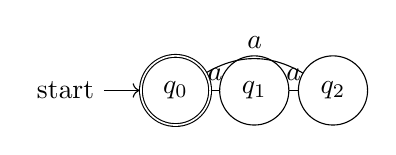
\begin{tikzpicture}
		\draw
			node[state,initial,accepting] (q0) {$q_0$}
			node[state,right of=q0]       (q1) {$q_1$}
			node[state,right of=q1]       (q2) {$q_2$}

			(q0) edge[above]            node{$a$} (q1)
			(q1) edge[above]            node{$a$} (q2)
			(q2) edge[above,bend right] node{$a$} (q0)
		;
    \end{tikzpicture}
\end{figure}

			\end{enumerate} \newpage

		\que{
			Transition of DFA which has strings of W with $|\text{W}| \mod 3$ and $|\text{W}| \mod 2$ can be
			obtained by taking the cross product of $\text{Q}_1$ \& $\text{Q}_2$ (Cartesian Product)
		}{~Find DFA with $\text{Q}=\{|\text{W}| : \text{W} \mod 3\} \times \{|\text{W}| : \text{W} \mod 2\}$}
		\ans
			\begin{enumerate}[label=Step \arabic* :,itemindent=\ansindent]
				\item Find Cartesian Product and identify states
					\begin{itemize}[label=]
						\item $\text{Q}_1=\{0,1,2\}$
						\item $\text{Q}_2=\{0,1\}$
						\item $\text{Q}_1 \times \text{Q}_2=\{(0,0),(0,1),(1,0),(1,1),(2,0),(2,1)\}$ \\
						\item For 5 states we have, $q_i \equiv (i \mod 3,i \mod 2)$
							\begin{itemize}[label=]
								\item $q_0 \equiv (0,0)$
								\item $q_1 \equiv (1,1)$
								\item $q_2 \equiv (2,0)$
								\item $q_3 \equiv (0,1)$
								\item $q_4 \equiv (1,0)$
								\item $q_5 \equiv (2,1)$
							\end{itemize}
					\end{itemize}
				\item Compute Transitions
				\begin{table}[H]
					\centering
					\begin{tabular}{cc}
						\begin{tabular}{c|c}
							$\delta$ & $a$ \\ \hline
							$q_0$ & $q_1$ \\
							$q_1$ & $q_2$ \\
							$q_2$ & $q_3$ \\
							$q_3$ & $q_4$ \\
							$q_4$ & $q_5$ \\
							$q_5$ & $q_0$
						\end{tabular} &
						\begin{tabular}{lll}
							$\delta(q_1,a)$ & $=$ & $q_2$ \\
							$\delta(q_2,a)$ & $=$ & $q_3$ \\
							$\delta(q_3,a)$ & $=$ & $q_4$ \\
							$\delta(q_4,a)$ & $=$ & $q_5$ \\
							$\delta(q_5,a)$ & $=$ & $q_0$
						\end{tabular}
					\end{tabular}
				\end{table}
				\item Final Design
					\begin{itemize}[leftmargin=2.5em]
						\item When $\text{W} \mod 3=\text{W} \mod 2$ \begin{figure}[H]
    \centering
    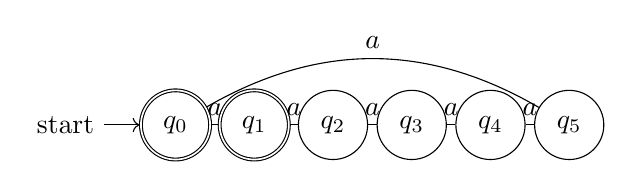
\begin{tikzpicture}
		\draw
			node [state,accepting,initial]     (q0) {$q_0$}
			node [state,accepting,right of=q0] (q1) {$q_1$}
			node [state,right of=q1]           (q2) {$q_2$}
			node [state,right of=q2]           (q3) {$q_3$}
			node [state,right of=q3]           (q4) {$q_4$}
			node [state,right of=q4]           (q5) {$q_5$}

			(q0) edge [above]            node{$a$} (q1)
			(q1) edge [above]            node{$a$} (q2)
			(q2) edge [above]            node{$a$} (q3)
			(q3) edge [above]            node{$a$} (q4)
			(q4) edge [above]            node{$a$} (q5)
			(q5) edge [above,bend right] node{$a$} (q0)
		;
    \end{tikzpicture}
\end{figure}

						\item When $\text{W} \mod 3\ne\text{W} \mod 2$ \begin{figure}[H]
    \centering
    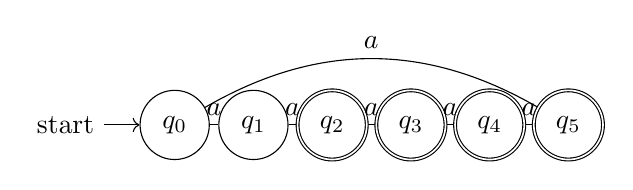
\begin{tikzpicture}
		\draw
			node[state,initial]               (q0) {$q_0$}
			node[state,right of=q0]           (q1) {$q_1$}
			node[state,accepting,right of=q1] (q2) {$q_2$}
			node[state,accepting,right of=q2] (q3) {$q_3$}
			node[state,accepting,right of=q3] (q4) {$q_4$}
			node[state,accepting,right of=q4] (q5) {$q_5$}

			(q0) edge[above]            node{$a$} (q1)
			(q1) edge[above]            node{$a$} (q2)
			(q2) edge[above]            node{$a$} (q3)
			(q3) edge[above]            node{$a$} (q4)
			(q4) edge[above]            node{$a$} (q5)
			(q5) edge[above,bend right] node{$a$} (q0)
		;
    \end{tikzpicture}
\end{figure}

						\item When $\text{W} \mod 3>\text{W} \mod 2$ \begin{figure}[H]
	\centering
	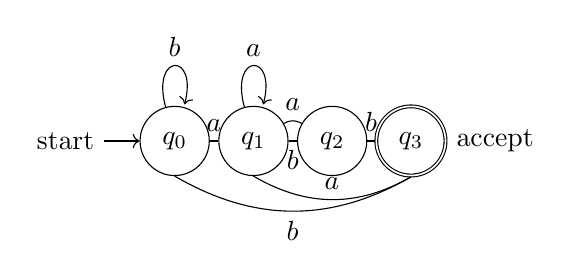
\begin{tikzpicture}
	\draw
		node [state,initial]                                  (q0) {$q_0$}
		node [state,right of=q0]                              (q1) {$q_1$}
		node [state,right of=q1]                              (q2) {$q_2$}
		node [state,accepting,right of=q2,label=right:accept] (q3) {$q_3$}
		(q0) edge[above] node{$a$} (q1)
		(q1) edge[below] node{$b$} (q2)
		(q2) edge[above] node{$b$} (q3)

		(q0) edge[loop above] node{$b$}            (q0)
		(q1) edge[loop above] node{$a$}            (q1)
		(q2) edge[bend right,above] node{$a$}      (q1)
		(q3.south) edge[bend left,above] node{$a$} (q1.south)
		(q3.south) edge[bend left,below] node{$b$} (q0.south)
	;
	\end{tikzpicture}
\end{figure}

					\end{itemize}
			\end{enumerate} \newpage

		\que{
			Obtain a DFA to accept language $\text{L}=\{\text{W} : |\text{W}| \mod 5 \ne 0\}$ on
			$\displaystyle\sum = \{a\}$
		}{~Accept language $\text{L}=\{\text{W} : |\text{W}| \mod 5 \ne 0\}$ on $\displaystyle \sum = \{a\}$}
		\ans
			\begin{enumerate}[label=Step \arabic* :,itemindent=\ansindent]
				\item Identify states
				\item Identify the number of states
					\begin{itemize}[label=]
						\item Remainder 0, the state is $q_0$
						\item Remainder 1, the state is $q_1$
						\item Remainder 2, the state is $q_2$
						\item Remainder 3, the state is $q_3$
						\item Remainder 4, the state is $q_4$
					\end{itemize}
				\item Identify the initial and accepting states
					\begin{itemize}[leftmargin=2.5em]
						\item In case of no input, the state is accepted
						\item In case of five or multiple of five input the state is accepted
					\end{itemize}
				\item Compute Transitions
					\begin{table}[H]
						\centering
						\begin{tabular}{cc}
							\begin{tabular}{l|l}
								$\delta$ & $a$ \\ \hline
								$q_0$ & $q_1$ \\
								$q_1$ & $q_2$ \\
								$q_2$ & $q_3$ \\
								$q_4$ & $q_0$ \\
							\end{tabular} &
							\begin{tabular}{lll}
								$\delta(q_0,a)$ & $=$ & $q_1$ \\
								$\delta(q_1,a)$ & $=$ & $q_2$ \\
								$\delta(q_2,a)$ & $=$ & $q_3$ \\
								$\delta(q_3,a)$ & $=$ & $q_4$ \\
								$\delta(q_4,a)$ & $=$ & $q_0$
							\end{tabular}
						\end{tabular}
					\end{table}
				\item Final Design \begin{figure}[H]
    \centering
    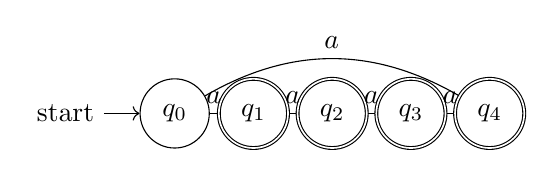
\begin{tikzpicture}
		\draw
			node [state,initial]               (q0) {$q_0$}
			node [state,accepting,right of=q0] (q1) {$q_1$}
			node [state,accepting,right of=q1] (q2) {$q_2$}
			node [state,accepting,right of=q2] (q3) {$q_3$}
			node [state,accepting,right of=q3] (q4) {$q_4$}

			(q0) edge [above] node{$a$} (q1)
			(q1) edge [above] node{$a$} (q2)
			(q2) edge [above] node{$a$} (q3)
			(q3) edge [above] node{$a$} (q4)
			(q4) edge [above,bend right] node{$a$} (q0)
		;
    \end{tikzpicture}
\end{figure}

			\end{enumerate} \newpage

		\que{Obtain a DFA to accept strings of $a$'s and $b$'s having even number of $a$'s and $b$'s}{
			Accept strings of $a$'s and $b$'s with even number of $a$'s and $b$'s
		}
		\ans
			\begin{enumerate}[label=Step \arabic* :,itemindent=\ansindent]
				\item Identify the number of states
				\indentpar{1.5em}{
					Since Even numbers can be 0 and multiple of 2 for 2 letters, there are 4 different states :
					\begin{itemize}[leftmargin=1.5em]
						\item Both $a$'s and $b$'s are even i.e $\text{E}_a\text{E}_b$
						\item Even $a$'s and odd $b$'s i.e $\text{E}_a\text{O}_b$
						\item Odd $a$'s and even $b$'s i.e $\text{O}_a\text{E}_b$
						\item Both $a$'s and $b$'s are odd i.e $\text{O}_a\text{O}_b$
					\end{itemize}
				}
				\item Identify the initial and accepting states
					\begin{itemize}[leftmargin=2.5em]
						\item In case of 0 or multiple of 2 input the state is accepted.
						\item All the rest of the cases are rejected.
					\end{itemize}
				\item Complete Transitions
					\begin{table}[H]
						\centering
						\begin{tabular}{cc}
							\begin{tabular}{c|c|c}
								$\delta$ & $a$ & $b$ \\ \hline
								$\text{E}_a\text{E}_b$ & $\text{O}_a\text{E}_b$ & $\text{E}_a\text{O}_b$ \\
								$\text{O}_a\text{E}_b$ & $\text{E}_a\text{E}_b$ & $\text{O}_a\text{O}_b$ \\
								$\text{E}_a\text{O}_b$ & $\text{O}_a\text{O}_b$ & $\text{E}_a\text{E}_b$ \\
								$\text{O}_a\text{O}_b$ & $\text{E}_a\text{O}_b$ & $\text{O}_a\text{E}_b$
							\end{tabular}
							\begin{tabular}{lll}
								$\delta(\text{E}_a\text{E}_b,a)$ & $=$ & $\text{O}_a\text{E}_b$ \\
								$\delta(\text{E}_a\text{E}_b,b)$ & $=$ & $\text{E}_a\text{O}_b$ \\
								$\delta(\text{O}_a\text{E}_b,a)$ & $=$ & $\text{E}_a\text{E}_b$ \\
								$\delta(\text{O}_a\text{E}_b,b)$ & $=$ & $\text{O}_a\text{O}_b$ \\
								$\delta(\text{E}_a\text{O}_b,a)$ & $=$ & $\text{O}_a\text{E}_b$ \\
								$\delta(\text{E}_a\text{O}_b,b)$ & $=$ & $\text{E}_a\text{E}_b$ \\
								$\delta(\text{O}_a\text{O}_b,b)$ & $=$ & $\text{E}_a\text{O}_b$ \\
								$\delta(\text{O}_a\text{O}_b,b)$ & $=$ & $\text{O}_a\text{E}_b$
							\end{tabular}
						\end{tabular}
					\end{table}
				\item Final Design % Select choices
% 1 - rounded  figure
% 2 - straight lines

\def \selection{1}

\begin{figure}[H]
    \centering
    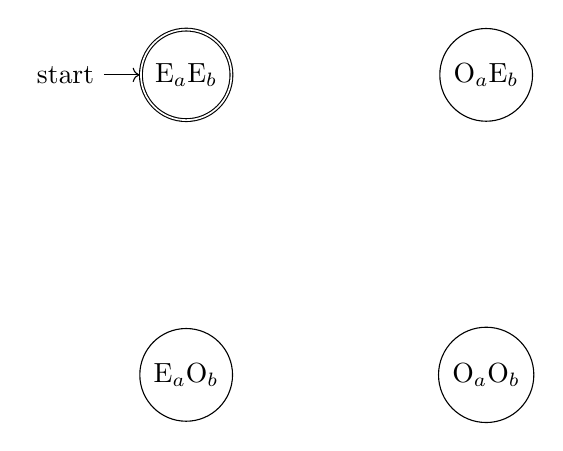
\begin{tikzpicture}[node distance=1.5in]
		\draw
			node [state,initial,accepting] (q0) {$\text{E}_a\text{E}_b$}
			node [state,right of=q0] (q1) {$\text{O}_a\text{E}_b$}
			node [state,below of=q0] (q2) {$\text{E}_a\text{O}_b$}
			node [state,right of=q2] (q3) {$\text{O}_a\text{O}_b$}

			\if \selection 1
				(q0.45-20)  edge [above] node{$a$} (q1.135+20)
				(q1.225-20) edge [below] node{$a$} (q0.315+20)
				(q2.45-20)  edge [above] node{$a$} (q3.135+20)
				(q3.225-20) edge [below] node{$a$} (q2.315+20)

				(q0.225+20) edge [left]  node{$b$} (q2.135-20)
				(q2.45+20)  edge [right] node{$b$} (q0.315-20)
				(q1.225+20) edge [left]  node{$b$} (q3.135-20)
				(q3.45+20)  edge [right] node{$b$} (q1.315-20)
			\fi

			\if \selection 2
				(q0) edge [<-,bend right,below] node{$a$} (q1)
				(q0) edge [<-,bend left,right]  node{$b$} (q2)
				(q2) edge [<-,bend right,below] node{$a$} (q3)
				(q1) edge [<-,bend right,left]  node{$b$} (q3)
				                                               
				(q0) edge [->,bend left,above] node{$a$} (q1)
				(q0) edge [->,bend right,left] node{$b$} (q2)
				(q2) edge [->,bend left,above] node{$a$} (q3)
				(q1) edge [->,bend left,right] node{$b$} (q3)
			\fi
		;
    \end{tikzpicture}
\end{figure}

			\end{enumerate}
	\end{enumerate} \newpage

	\subsection{Definite Finite State Machines}
	\begin{enumerate}[label=\arabic*)]
		\que{
			NDFA to accept pairs strings of $a$'s and $b$'s ending with $ab$ and moves made for sequence of
			$abaab$ and $abb$
		}{~Accept NDFA for strings ending with $ab$ and moves made for sequence $abaab$ and $abb$}
		\ans
			\begin{enumerate}[label=Step \arabic* :,itemindent=\ansindent]
				\item Minimum String is `$ab$'
				\item Alphabets $$\sum=\{a\}$$
				\item Skeleton DFA \begin{figure}[H]
	\centering
	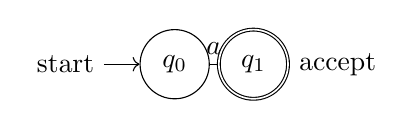
\begin{tikzpicture}
		\draw
			node[state,initial]                                  (q0) {$q_0$}
			node[state,accepting,right of=q0,label=right:accept] (q1) {$q_1$}

			(q0) edge[above] node{$a$} (q1)
		;
	\end{tikzpicture}
\end{figure}

				\item Compute Transitions
					\begin{table}[H]
						\centering
						\begin{tabular}{cc}
							\begin{tabular}{c|c|c}
								$\delta$ & $a$ & $b$ \\ \hline
								$q_0$ & $\{q_0,q_1\}$ & $q_0$ \\
								$q_1$ & $\varnothing$ & $q_2$ \\
								$q_2$ & $\varnothing$ & $\varnothing$
							\end{tabular}
						\end{tabular}
					\end{table}
				\item Final NDFA \begin{figure}[H]
	\centering
	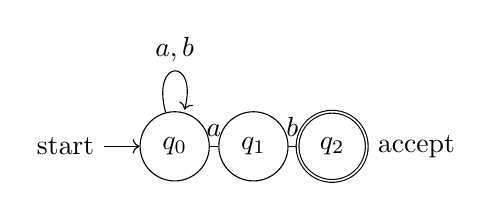
\begin{tikzpicture}
		\draw
			node[state,initial]                                  (q0) {$q_0$}
			node[state,right of=q0]                              (q1) {$q_1$}
			node[state,accepting,right of=q1,label=right:accept] (q2) {$q_2$}

			(q0) edge[above]      node{$a$}   (q1)
			(q0) edge[loop above] node{$a,b$} (q1)
			(q1) edge[above]      node{$b$}   (q2)
		;
	\end{tikzpicture}
\end{figure}

				\item Moves made for
					\begin{itemize}
						\item $abaab$ \begin{figure}[H]
	\centering
	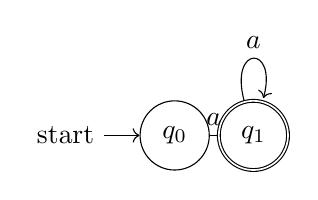
\begin{tikzpicture}
	\draw
		node [state,initial]               (q0) {$q_0$}
		node [state,accepting,right of=q0] (q1) {$q_1$}
		(q0) edge[above] node{$a$}         (q1)
		(q1) edge[loop above] node{$a$}    (q1)
	;
	\end{tikzpicture}
\end{figure}

						\item $abb$ \def \sequence{a,b,b}

\begin{figure}[H]
	\centering
	\begin{tikzpicture}[node distance=.75in]
		\draw
			node[state,initial]   (0) {$q_0$}

			\foreach[count=\j] \i in {1,...,3}{
				node[state,right of=\the \numexpr \j - 1 \relax] (\j) {$q_0$}
			}

			node[state,below right of=0]           (5) {$q_1$}
			node[state,accepting,below right of=6] (6) {$q_2$}

			\foreach[count=\j] \i in \sequence{
				(\the \numexpr \j - 1 \relax) edge[above] node{$\i$} (\j)
			}

			(0) edge[above right] node{$a$} (5)
			(5) edge[above right] node{$b$} (6)
		;
	\end{tikzpicture}
\end{figure}

					\end{itemize}
			\end{enumerate} \newpage

		\que{
			Obtain an NDFA to accept the following language
			$\text{L}=\{\text{W} : \text{W}\in ababa \text{ or } abab^n\}$
		}{~Accept language $\text{L}=\{\text{W} : \text{W}\in ababa \text{ or } abab^n\}$}
		\ans
			\begin{enumerate}[label=Step \arabic* :,itemindent=\ansindent]
				\item Minimum string is `$ab$'
				\item Alphabets $$\sum=\{a,b\}$$
				\item Skeleton NDFA's \begin{figure}[H]
	\centering
	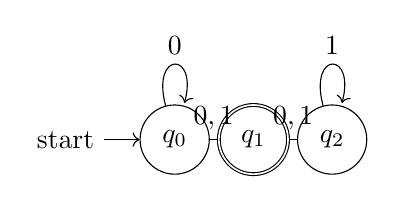
\begin{tikzpicture}
		\draw
			node[state,initial]               (q0) {$q_0$}
			node[state,accepting,right of=q0] (q1) {$q_1$}
			node[state,right of=q1]           (q2) {$q_2$}

			(q0) edge[loop above] node{$0$}   (q0)
			(q2) edge[loop above] node{$1$}   (q2)
			(q0) edge[above]      node{$0,1$} (q1)
			(q1) edge[above]      node{$0,1$} (q2)
		;
	\end{tikzpicture}
\end{figure}

				\item Combining Transitions
					\indentpar{1.5em}{Combining first states from skeletons i.e $q_0$, $q_4$ as $q_0$}
					\begin{table}[H]
						\centering
						\begin{tabular}{cc}
							\begin{tabular}{c|c|c}
								$\delta$ & $a$           & $b$           \\ \hline
								$q_0$    & $\{q_1,q_5\}$ & $\varnothing$ \\
								$q_1$    & $\varnothing$ & $q_2$         \\
								$q_2$    & $q_3$         & $\varnothing$ \\
								$q_3$    & $\varnothing$ & $q_3$         \\
								$q_5$    & $\varnothing$ & $q_6$         \\
								$q_6$    & $q_6$         & $\varnothing$
							\end{tabular} &
							\begin{tabular}{lll}
								$\delta(q_0,a)$ & $=$ & $\{q_1,q_5\}$ \\
								$\delta(q_1,b)$ & $=$ & $q_2$         \\
								$\delta(q_2,a)$ & $=$ & $q_3$         \\
								$\delta(q_3,b)$ & $=$ & $q_3$         \\
								$\delta(q_5,b)$ & $=$ & $q_6$         \\
								$\delta(q_6,a)$ & $=$ & $q_6$
							\end{tabular}
						\end{tabular}
					\end{table}
				\item Final NDFA \begin{figure}[H]
	\centering
	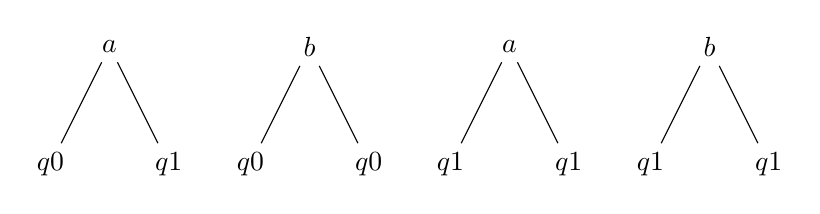
\begin{tikzpicture}[node distance=1in]
		\draw
			node (0) {$a$}
				child {node {$q0$}}
				child {node {$q1$}}

			node[right of=0] (0) {$b$}
				child {node {$q0$}}
				child {node {$q0$}}

			node[right of=0] (0) {$a$}
				child {node {$q1$}}
				child {node {$q1$}}

			node[right of=0] (0) {$b$}
				child {node {$q1$}}
				child {node {$q1$}}
		;
	\end{tikzpicture}
\end{figure}

			\end{enumerate} \newpage

		\que{Design an NDFA to recognize following set of strings $abc$, $abd$ \& $aacd$}{
			Design ae NDFA to recognize strings $abc$, $abd$ \& $aacd$
		}
		\ans
			\begin{enumerate}[label=Step \arabic* :,itemindent=\ansindent]
				\item Minimum strings are $abc$, $abd$ and $aacd$
				\item Alphabets $$\sum=\{a,b,c,d\}$$
				\item Skeleton NDFA's \begin{figure}[H]
	\centering
	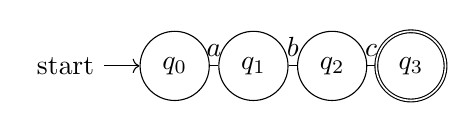
\begin{tikzpicture}
		\draw
			node[state,initial]               (q0) {$q_0$}
			node[state,right of=q0]           (q1) {$q_1$}
			node[state,right of=q1]           (q2) {$q_2$}
			node[state,accepting,right of=q2] (q3) {$q_3$}

			(q0) edge[above] node{$a$} (q1)
			(q1) edge[above] node{$b$} (q2)
			(q2) edge[above] node{$c$} (q3)
		;
	\end{tikzpicture} \\
	$abc$
\end{figure}

\begin{figure}[H]
	\centering
	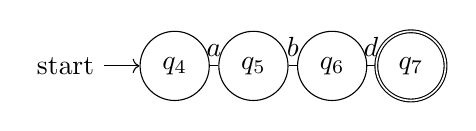
\begin{tikzpicture}
		\draw
			node[state,initial]               (q4) {$q_4$}
			node[state,right of=q4]           (q5) {$q_5$}
			node[state,right of=q5]           (q6) {$q_6$}
			node[state,accepting,right of=q6] (q7) {$q_7$}

			(q4) edge[above] node{$a$} (q5)
			(q5) edge[above] node{$b$} (q6)
			(q6) edge[above] node{$d$} (q7)
		;
	\end{tikzpicture} \\
	$abd$
\end{figure}

\begin{figure}[H]
	\centering
	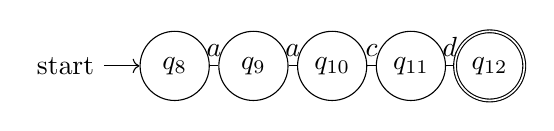
\begin{tikzpicture}
		\draw
			node[state,initial]                (q8)  {$q_8$}
			node[state,right of=q8]            (q9)  {$q_9$}
			node[state,right of=q9]            (q10) {$q_{10}$}
			node[state,right of=q10]           (q11) {$q_{11}$}
			node[state,accepting,right of=q11] (q12) {$q_{12}$}

			(q8)  edge[above] node{$a$} (q9)
			(q9)  edge[above] node{$a$} (q10)
			(q10) edge[above] node{$c$} (q11)
			(q11) edge[above] node{$d$} (q12)
		;
	\end{tikzpicture} \\
	$aacd$
\end{figure}

				\item Combining Transitions
					\indentpar{1.5em}{Combining first states from skeletons i.e $q_0$, $q_4$ and $q_8$ as $q_0$}
					\begin{table}[H]
						\centering
						\begin{tabular}{cc}
							\begin{tabular}{c|c|c|c|c}
								$\delta$ & $a$ & $b$ & $c$ & $d$ \\ \hline
								$q_0$ & $\{q_1,q_5,q_9\}$ & $\varnothing$ & $\varnothing$ & $\varnothing$ \\
								$q_1$ & $\varnothing$ & $q_2$ & $\varnothing$ & $\varnothing$ \\
								$q_2$ & $\varnothing$ & $\varnothing$ & $q_3$ & $\varnothing$ \\
								$q_3$ & $\varnothing$ & $\varnothing$ & $\varnothing$ & $\varnothing$ \\
								$q_5$ & $\varnothing$ & $q_6$ & $\varnothing$ & $\varnothing$ \\
								$q_6$ & $\varnothing$ & $\varnothing$ & $\varnothing$ & $q_7$ \\
								$q_7$ & $\varnothing$ & $\varnothing$ & $\varnothing$ & $\varnothing$ \\
								$q_9$ & $q_{10}$ & $\varnothing$ & $\varnothing$ & $\varnothing$ \\
								$q_{10}$ & $\varnothing$ & $\varnothing$ & $q_{11}$ & $\varnothing$ \\
								$q_{11}$ & $\varnothing$ & $\varnothing$ & $\varnothing$ & $q_{12}$ \\
								$q_{12}$ & $\varnothing$ & $\varnothing$ & $\varnothing$ & $\varnothing$
							\end{tabular} &
							\begin{tabular}{lll}
								$\delta(q_0,a)$ & $=$ & $\{q_1,q_5,q_9\}$ \\
								$\delta(q_1,b)$ & $=$ & $q_2$ \\
								$\delta(q_2,c)$ & $=$ & $q_3$ \\
								$\delta(q_5,b)$ & $=$ & $q_6$ \\
								$\delta(q_6,d)$ & $=$ & $q_7$ \\
								$\delta(q_9,a)$ & $=$ & $q_{10}$ \\
								$\delta(q_{10},c)$ & $=$ & $q_{11}$ \\
								$\delta(q_{11},d)$ & $=$ & $q_{12}$
							\end{tabular}
						\end{tabular}
					\end{table}
				\item Final NDFA \begin{figure}[H]
	\centering
	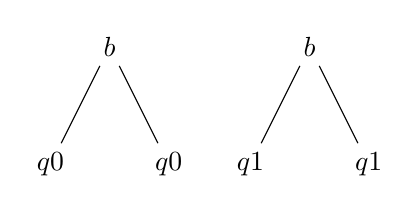
\begin{tikzpicture}[node distance=1in]
		\draw
			node (0) {$b$}
				child {node {$q0$}}
				child {node {$q0$}}

			node[right of=0] (0) {$b$}
				child {node {$q1$}}
				child {node {$q1$}}
		;
	\end{tikzpicture}
\end{figure}

			\end{enumerate} \newpage

		\que{Design an NDFA to recognize following set of strings 0101, 101 \& 011}{
			Design ae NDFA to recognize strings 0101, 101 \& 011
		}
		\ans
			\begin{enumerate}[label=Step \arabic* :,itemindent=\ansindent]
				\item Minimum strings are 0101, 101 and 011
				\item Alphabets $$\sum=\{0,1\}$$
				\item Skeleton NDFA's \begin{figure}[H]
	\centering
	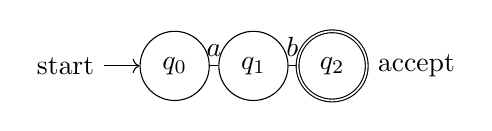
\begin{tikzpicture}
	\draw
		node [state,initial]                                  (q0) {$q_0$}
		node [state,right of=q0]                              (q1) {$q_1$}
		node [state,accepting,right of=q1,label=right:accept] (q2) {$q_2$}
		(q0) edge[above] node{$a$}                            (q1)
		(q1) edge[above] node{$b$}                            (q2)
	;
	\end{tikzpicture}
\end{figure}

				\item Combining Transitions
					\indentpar{1.5em}{Combining first states from skeletons i.e $q_0$, $q_5$ and $q_9$ as $q_0$}
					\begin{table}[H]
						\centering
						\begin{tabular}{cc}
							\begin{tabular}{c|c|c}
								$\delta$ & $0$ & $1$ \\ \hline
								$q_0$ & $\{q_1,q_{10}\}$ & $q_6$ \\
								$q_1$ & $\varnothing$ & $q_2$ \\
								$q_2$ & $q_3$ & $\varnothing$ \\
								$q_3$ & $\varnothing$ & $q_4$ \\
								$q_4$ & $\varnothing$ & $\varnothing$ \\
								$q_6$ & $q_7$ & $\varnothing$ \\
								$q_7$ & $\varnothing$ & $q_8$ \\
								$q_8$ & $\varnothing$ & $\varnothing$ \\
								$q_{10}$ & $\varnothing$ & $q_{11}$ \\
								$q_{11}$ & $\varnothing$ & $q_{12}$ \\
								$q_{12}$ & $\varnothing$ & $\varnothing$
							\end{tabular} &
							\begin{tabular}{lll}
								$\delta(q_0,0)$ & $=$ & $\{q_1,q_{10}\}$ \\
								$\delta(q_0,1)$ & $=$ & $q_6$ \\
								$\delta(q_1,1)$ & $=$ & $q_2$ \\
								$\delta(q_2,0)$ & $=$ & $q_3$ \\
								$\delta(q_3,1)$ & $=$ & $q_4$ \\
								$\delta(q_6,0)$ & $=$ & $q_7$ \\
								$\delta(q_7,1)$ & $=$ & $q_8$ \\
								$\delta(q_{10},1)$ & $=$ & $q_{11}$ \\
								$\delta(q_{11},1)$ & $=$ & $q_{12}$
							\end{tabular}
						\end{tabular}
					\end{table}
				\item Final NDFA's \begin{figure}[H]
	\centering
	\begin{tikzpicture}
		\draw
			node[state,initial]                (q0) {$q_0$}
			node[state,above right of=q0]      (q1) {$q_1$}
			node[state,right of=q1]            (q2) {$q_2$}
			node[state,right of=q2]            (q3) {$q_3$}
			node[state,accepting,right of=q3]  (q4) {$q_4$}

			node[state,below right of=q0]      (q6) {$q_6$}
			node[state,right of=q6]            (q7) {$q_7$}
			node[state,accepting,right of=q7]  (q8) {$q_8$}

			node[state,right of=q0]            (q10) {$q_{10}$}
			node[state,right of=q10]           (q11) {$q_{11}$}
			node[state,accepting,right of=q11] (q12) {$q_{12}$}

			(q0)  edge[above left] node{$0$} (q1)
			(q1)  edge[above]      node{$1$} (q2)
			(q2)  edge[above]      node{$0$} (q3)
			(q3)  edge[above]      node{$1$} (q4)

			(q0)  edge[above]      node{$0$} (q10)
			(q6)  edge[above]      node{$0$} (q7)
			(q7)  edge[above]      node{$1$} (q8)

			(q0)  edge[below left] node{$1$} (q6)
			(q10) edge[above]      node{$1$} (q11)
			(q11) edge[above]      node{$1$} (q12)
		;
	\end{tikzpicture}
\end{figure}


			\end{enumerate}
	\end{enumerate} \newpage

	\subsection{Conversion of DFA to NDFA by Subset Construction}
	\begin{enumerate}[label=\arabic*)]
		\que{
			Obtain the DFA for the following NDFA by Subset Construction method \begin{figure}[H]
	\centering
	\begin{tikzpicture}
		\draw
			node[state,initial]                                  (q0) {$q_0$}
			node[state,accepting,right of=q0,label=right:accept] (q1) {$q_1$}

			(q0) edge[above] node{$a$} (q1)
		;
	\end{tikzpicture}
\end{figure}

		}{
			Obtain DFA for given NDFA by Subset Construction method
		}
		\ans
			\begin{enumerate}[label=Step \arabic* :,itemindent=\ansindent]
				\item Find Transitions
					\begin{table}[H]
						\centering
						\begin{tabular}{c|c|c}
							$\delta$ & $a$ & $b$ \\ \hline
							$q_0$ & $\{q_0,q_1\}$ & $q_0$ \\
							$q_1$ & $\varnothing$ & $q_2$ \\
							$q_2$ & $\varnothing$ & $\varnothing$
						\end{tabular}
					\end{table}
				\item Identify initial and accepting state
					\begin{itemize}[label=,leftmargin=1.5em]
						\item $\text{F}_0 = \{q_2,\{q_0,q_2\},\{q_0,q_1,q_2\}\}$
						\item $\text{F}_n = q_2$
					\end{itemize}
				\item Identify transitions for all possible subests
					\begin{table}[H]
						\centering
						\begin{tabular}{cc}
							\begin{tabular}{c|c|c}
								$\delta$          & $a$           & $b$           \\ \hline
								$q_0$             & $\{q_0,q_1\}$ & $q_0$         \\
								$q_1$             & $\varnothing$ & $q_2$         \\
								$q_2$             & $\varnothing$ & $\varnothing$ \\
								$\{q_0,q_1\}$     & $\{q_0,q_1\}$ & $\{q_0,q_2\}$ \\
								$\{q_1,q_2\}$     & $\varnothing$ & $q_2$         \\
								$\{q_2,q_0\}$     & $\{q_0,q_1\}$ & $q_0$         \\
								$\{q_0,q_1,q_2\}$ & $\{q_0,q_1\}$ & $\{q_0,q_2\}$
							\end{tabular} &
							\begin{tabular}{clc}
								$\delta(q_0,a)$             & $=$ & $\{q_0,q_1\}$ \\
								$\delta(q_0,b)$             & $=$ & $q_0$         \\
								$\delta(q_1,b)$             & $=$ & $q_2$         \\
								$\delta(\{q_0,q_1\},a)$     & $=$ & $\{q_0,q_1\}$ \\
								$\delta(\{q_0,q_1\},b)$     & $=$ & $\{q_0,q_2\}$ \\
								$\delta(\{q_1,q_2\},b)$     & $=$ & $q_2$         \\
								$\delta(\{q_2,q_0\},a)$     & $=$ & $\{q_0,q_1\}$ \\
								$\delta(\{q_0,q_2\},b)$     & $=$ & $q_0$         \\
								$\delta(\{q_0,q_1,q_2\},a)$ & $=$ & $\{q_0,q_1\}$ \\
								$\delta(\{q_0,q_1,q_2\},b)$ & $=$ & $\{q_0,q_2\}$
							\end{tabular}
						\end{tabular}
					\end{table}
					\item Convert transitions to DFA
						\indentpar{1.5em}{Replace Similar elements with a letter}
						\begin{table}[H]
							\centering
							\begin{tabular}{c|c|c}
								$\delta$     & $a$                & $b$                \\ \hline
						\hltt	$\text{A}_0$ & \hltt $\text{A}_3$ & \hltt $\text{A}_0$ \\
								$\text{A}_1$ & $\varnothing$      & $\text{A}_2$       \\
								$\text{A}_2$ & $\varnothing$      & $\varnothing$      \\
						\hltt	$\text{A}_3$ & \hltt $\text{A}_3$ & \hltt $\text{A}_5$ \\
								$\text{A}_4$ & $\varnothing$      & $\text{A}_2$       \\
						\hltt	$\text{A}_5$ & \hltt $\text{A}_3$ & \hltt $\text{A}_0$ \\
								$\text{A}_6$ & $\text{A}_3$       & $\text{A}_5$
							\end{tabular}
						\end{table}
				\item Final DFA \begin{figure}[H]
	\centering
	\begin{tikzpicture}
		\draw
			node[state,initial]                                  (q0) {$q_0$}
			node[state,right of=q0]                              (q1) {$q_1$}
			node[state,accepting,right of=q1,label=right:accept] (q2) {$q_2$}

			(q0) edge[above]      node{$a$}   (q1)
			(q0) edge[loop above] node{$a,b$} (q1)
			(q1) edge[above]      node{$b$}   (q2)
		;
	\end{tikzpicture}
\end{figure}

			\end{enumerate}
	\end{enumerate} \newpage

	\subsection{Conversion of DFA to NDFA by Lazy Evaluation}
	\begin{enumerate}[label=\arabic*)]
		\que{Obtain the DFA for the following NDFA by Lazy evaluation method \begin{figure}[H]
	\centering
	\begin{tikzpicture}
		\draw
			node[state,initial]               (q0) {$q_0$}
			node[state,accepting,right of=q0] (q1) {$q_1$}
			node[state,right of=q1]           (q2) {$q_2$}

			(q0) edge[loop above] node{$0$}   (q0)
			(q2) edge[loop above] node{$1$}   (q2)
			(q0) edge[above]      node{$0,1$} (q1)
			(q1) edge[above]      node{$0,1$} (q2)
		;
	\end{tikzpicture}
\end{figure}
}{
			Obtain the DFA for the following NDFA by Lazy evaluation method
		}
		\ans
			\begin{enumerate}[label=Step \arabic* :,itemindent=\ansindent]
				\item Find Transitions
					\begin{table}[H]
						\centering
						\begin{tabular}{c|c|c}
							$\delta$ & 0             & 1     \\ \hline
							$q_0$    & $\{q_0,q_1\}$ & $q_1$ \\
							$q_1$    & $q_2$         & $q_2$ \\
							$q_2$    & $\varnothing$ & $q_2$
						\end{tabular}
					\end{table}
				\item Identify initial and accepting state
					\begin{itemize}[label=,leftmargin=1.5em]
						\item $\text{F}_0=\{q_2,\{q_0,q_2\},\{q_0,q_1,q_2\}\}$
						\item $\text{F}_1=q_2$
					\end{itemize}
				\item Identify transitions for all possible subsets
					\begin{table}[H]
						\centering
						\begin{tabular}{cc}
							\begin{tabular}{c|c|c}
								$\delta$          & 0                 & 1             \\ \hline
								$q_0$             & $\{q_0,q_1\}$     & $q_1$         \\
								$q_1$             & $q_2$             & $q_2$         \\
								$q_2$             & $\varnothing$     & $q_2$         \\
								$\{q_0,q_1\}$     & $\{q_0,q_1,q_2\}$ & $\{q_1,q_2\}$ \\
								$\{q_1,q_2\}$     & $q_2$             & $q_2$         \\
								$\{q_0,q_2\}$     & $\{q_0,q_1\}$     & $\{q_1,q_2\}$ \\
								$\{q_0,q_1,q_2\}$ & $\{q_0,q_1,q_2\}$ & $\{q_1,q_2\}$
							\end{tabular} &
							\begin{tabular}{ccc}
								$\delta(q_0,0)$             & $=$ & $\{q_0,q_1\}$     \\
								$\delta(q_0,1)$             & $=$ & $q_1$             \\
								$\delta(q_1,0)$             & $=$ & $q_2$             \\
								$\delta(q_1,1)$             & $=$ & $q_2$             \\
								$\delta(q_2,1)$             & $=$ & $q_2$             \\
								$\delta(\{q_0,q_1\},0)$     & $=$ & $\{q_0,q_1,q_2\}$ \\
								$\delta(\{q_0,q_1\},1)$     & $=$ & $\{q_1,q_2\}$     \\
								$\delta(\{q_1,q_2\},0)$     & $=$ & $q_2$             \\
								$\delta(\{q_1,q_2\},1)$     & $=$ & $q_2$             \\
								$\delta(\{q_0,q_2\},0)$     & $=$ & $\{q_0,q_1\}$     \\
								$\delta(\{q_0,q_2\},1)$     & $=$ & $\{q_1,q_2\}$     \\
								$\delta(\{q_0,q_1,q_2\},0)$ & $=$ & $\{q_1,q_2\}$     \\
								$\delta(\{q_0,q_1,q_2\},1)$ & $=$ & $\{q_1,q_2\}$
							\end{tabular}
						\end{tabular}
					\end{table}
				\item Convert transitions to DFA
					\indentpar{1.5em}{Replace Similar elements with a letter}
					\begin{table}[H]
						\centering
						\begin{tabular}{c|c|c}
							$\delta$          & 0                       & 1                   \\ \hline
					\hltt	$q_0$             & $\{q_0,q_1\}$           & $q_1$               \\
					\hltt	$\{q_0,q_1\}$     & $\{q_0,q_1,q_2\}$       & $\{q_1,q_2\}$       \\
					\hltt	$q_1$             & $q_2$                   & $q_2$               \\
					\hltt	$\{q_0,q_1,q_2\}$ & \hltt $\{q_0,q_1,q_2\}$ & \hltt $\{q_1,q_2\}$ \\
					\hltt	$\{q_1,q_2\}$     & \hltt $q_2$             & \hltt	$q_2$         \\
					\hltt	$q_2$             & $\varnothing$           & \hltt	$q_2$
						\end{tabular}
					\end{table} \newpage
				\item Final DFA \begin{figure}[H]
	\centering
	\begin{tikzpicture}[node distance=1in]
		\draw
			node (0) {$a$}
				child {node {$q0$}}
				child {node {$q1$}}

			node[right of=0] (0) {$b$}
				child {node {$q0$}}
				child {node {$q0$}}

			node[right of=0] (0) {$a$}
				child {node {$q1$}}
				child {node {$q1$}}

			node[right of=0] (0) {$b$}
				child {node {$q1$}}
				child {node {$q1$}}
		;
	\end{tikzpicture}
\end{figure}

			\end{enumerate}
	\end{enumerate} \newpage
\end{document}
